\documentclass[border=2pt]{standalone}
\usepackage{newtxtext,newtxmath}
\usepackage{tikz,pgfplots,amsmath}
\usetikzlibrary{arrows.meta,positioning,calc,shapes.geometric}
\pgfplotsset{compat=1.18}
\definecolor{navy}{HTML}{24465E}
\definecolor{teal}{HTML}{327F83}
\definecolor{coral}{HTML}{BF594C}
\definecolor{ochre}{HTML}{AC7A28}
\definecolor{slate}{HTML}{67737D}
\definecolor{mist}{HTML}{E4E9EC}
\definecolor{pale}{HTML}{F4F7F8}
\definecolor{wine}{HTML}{885878}
\definecolor{lightteal}{HTML}{E3F0EF}
\tikzset{every node/.style={font=\sffamily\fontsize{8}{9.5}\selectfont},
 block/.style={draw=slate!65,fill=pale,rounded corners=1.5pt,inner sep=5pt,align=center},
 link/.style={-{Latex[length=1.8mm,width=1.15mm]},draw=slate,line width=.65pt}}
\pgfplotsset{every axis/.append style={
 font=\sffamily\fontsize{8}{9.5}\selectfont,
 tick label style={font=\sffamily\fontsize{7}{8.3}\selectfont,/pgf/number format/fixed,/pgf/number format/precision=3},
 label style={font=\sffamily\fontsize{8}{9.5}\selectfont},
 axis line style={slate!70,line width=.45pt},tick style={slate!70},
 grid style={mist,line width=.35pt},
 legend style={font=\sffamily\fontsize{7}{8.2}\selectfont,draw=none,fill=white,cells={anchor=west}},
 scaled ticks=false,clip=true,mark size=1.6pt}}

\begin{document}
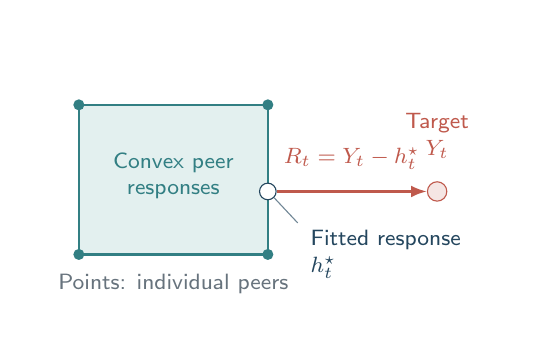
\begin{tikzpicture}

\path[use as bounding box] (-.65,-.7) rectangle (5.55,2.88);
\filldraw[draw=teal,fill=lightteal,line width=.8pt] (0,0)--(2.4,0)--(2.4,1.9)--(0,1.9)--cycle;
\foreach \x/\y in {0/0,2.4/0,2.4/1.9,0/1.9}{\fill[teal] (\x,\y) circle (2pt);}
\node[text=teal,align=center,text width=2.0cm] at (1.2,1.0) {Convex peer\\responses};
\node[circle,draw=navy,fill=white,inner sep=0pt,minimum size=6pt] (h) at (2.4,.80) {};
\node[circle,draw=coral,fill=coral!15,inner sep=0pt,minimum size=7pt] (t) at (4.55,.80) {};
\draw[-{Latex[length=2mm]},coral,line width=.95pt] (h.east)--node[above=4pt,text=coral] {$R_t=Y_t-h_t^\star$} (t.west);
\draw[navy!65,line width=.4pt] (h.south east)--(2.78,.40);
\node[anchor=north west,align=left,text=navy] at (2.82,.43) {Fitted response\\$h_t^\star$};
\node[anchor=south,align=center,text=coral] at (4.55,1.1) {Target\\$Y_t$};
\node[anchor=north,text=slate] at (1.2,-.12) {Points: individual peers};

\end{tikzpicture}
\end{document}
